\section{Breaking waves}
In accordance to [N3], wave breaking (or wave slamming) as a consequence of steep irregular sea states shall be considered in the design of offshore substructures. As criteria, the exceedance of 0.04 by the ratio of significant wave height $H_{S}$ and wave length $\lambda$ is given.

\begin{align}
H_{S} / L\left(T_{p}\right)>0.04
\end{align}

The wave length $L$ is given by the linear dispersion relationship based on the peak period $T_{p}$ of the sea state.\\

\begin{figure}[H] 
 \centering 
 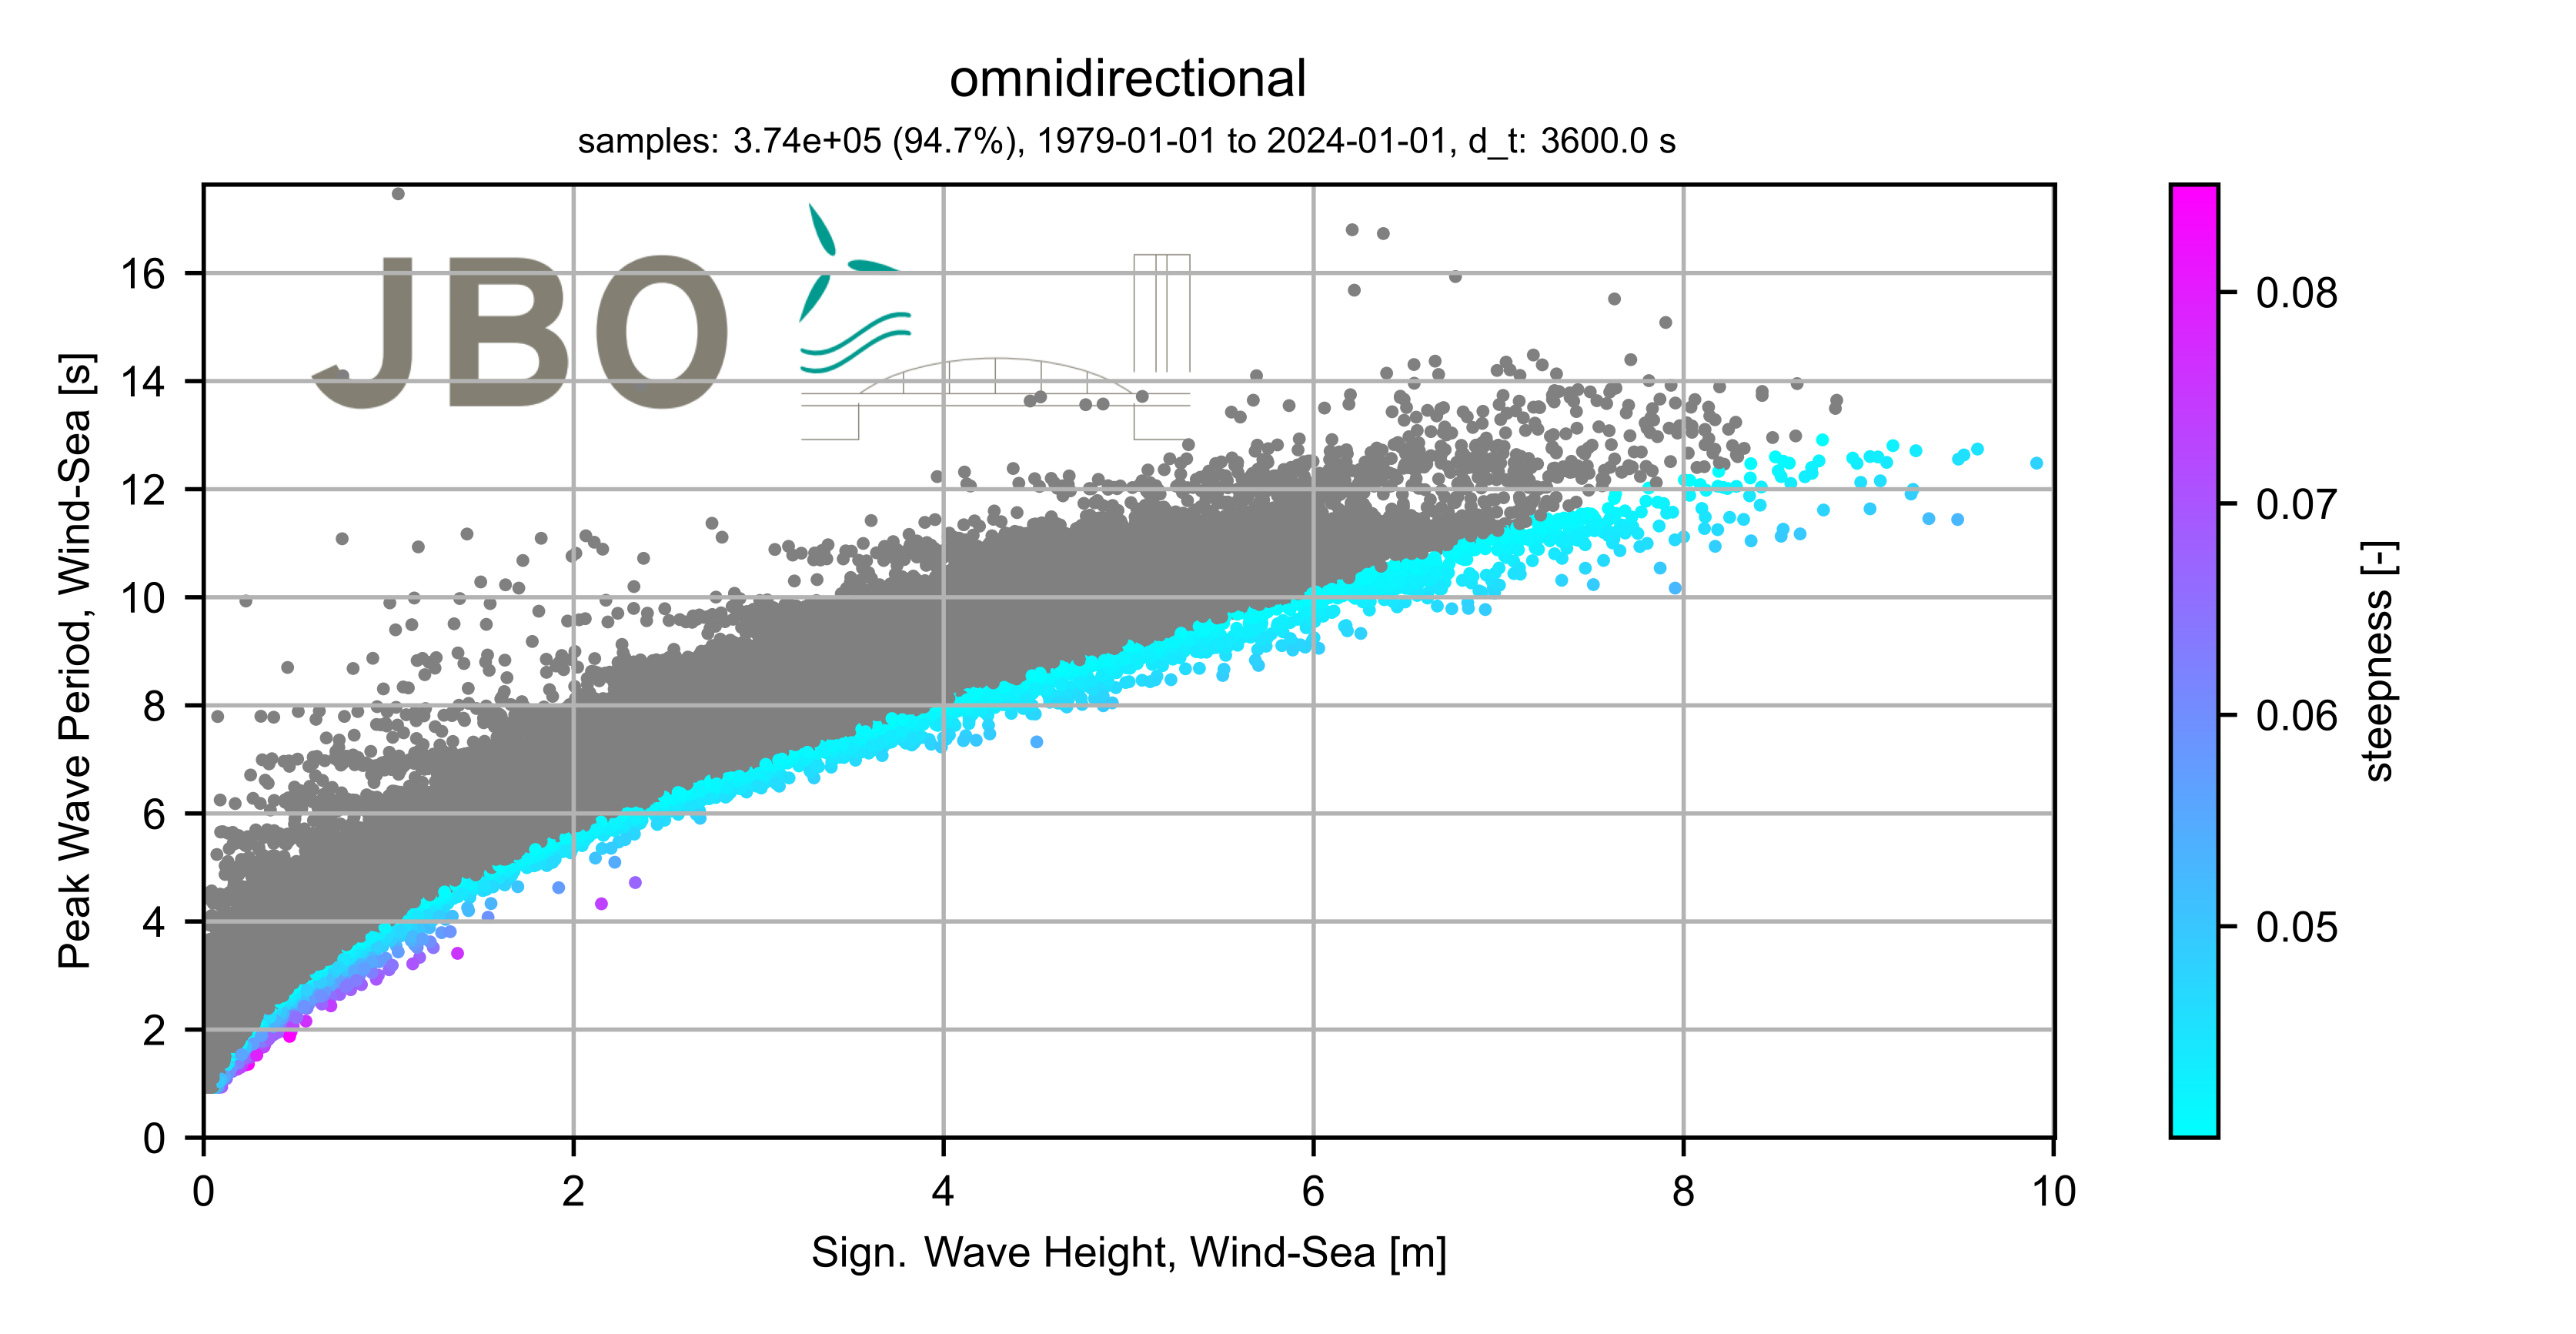
\includegraphics[width=1.0\textwidth]{C:/Users/aaron.lange/Desktop/Projekte/Hindcast_Tool/HindTool/example_output/WaveBreak_wind_page_3.png} 
 \caption{ WaveBreak-wind-page-3 } 
 \label{fig: WaveBreak_wind_page_3 } 
\end{figure}


\begin{figure}[H] 
 \centering 
 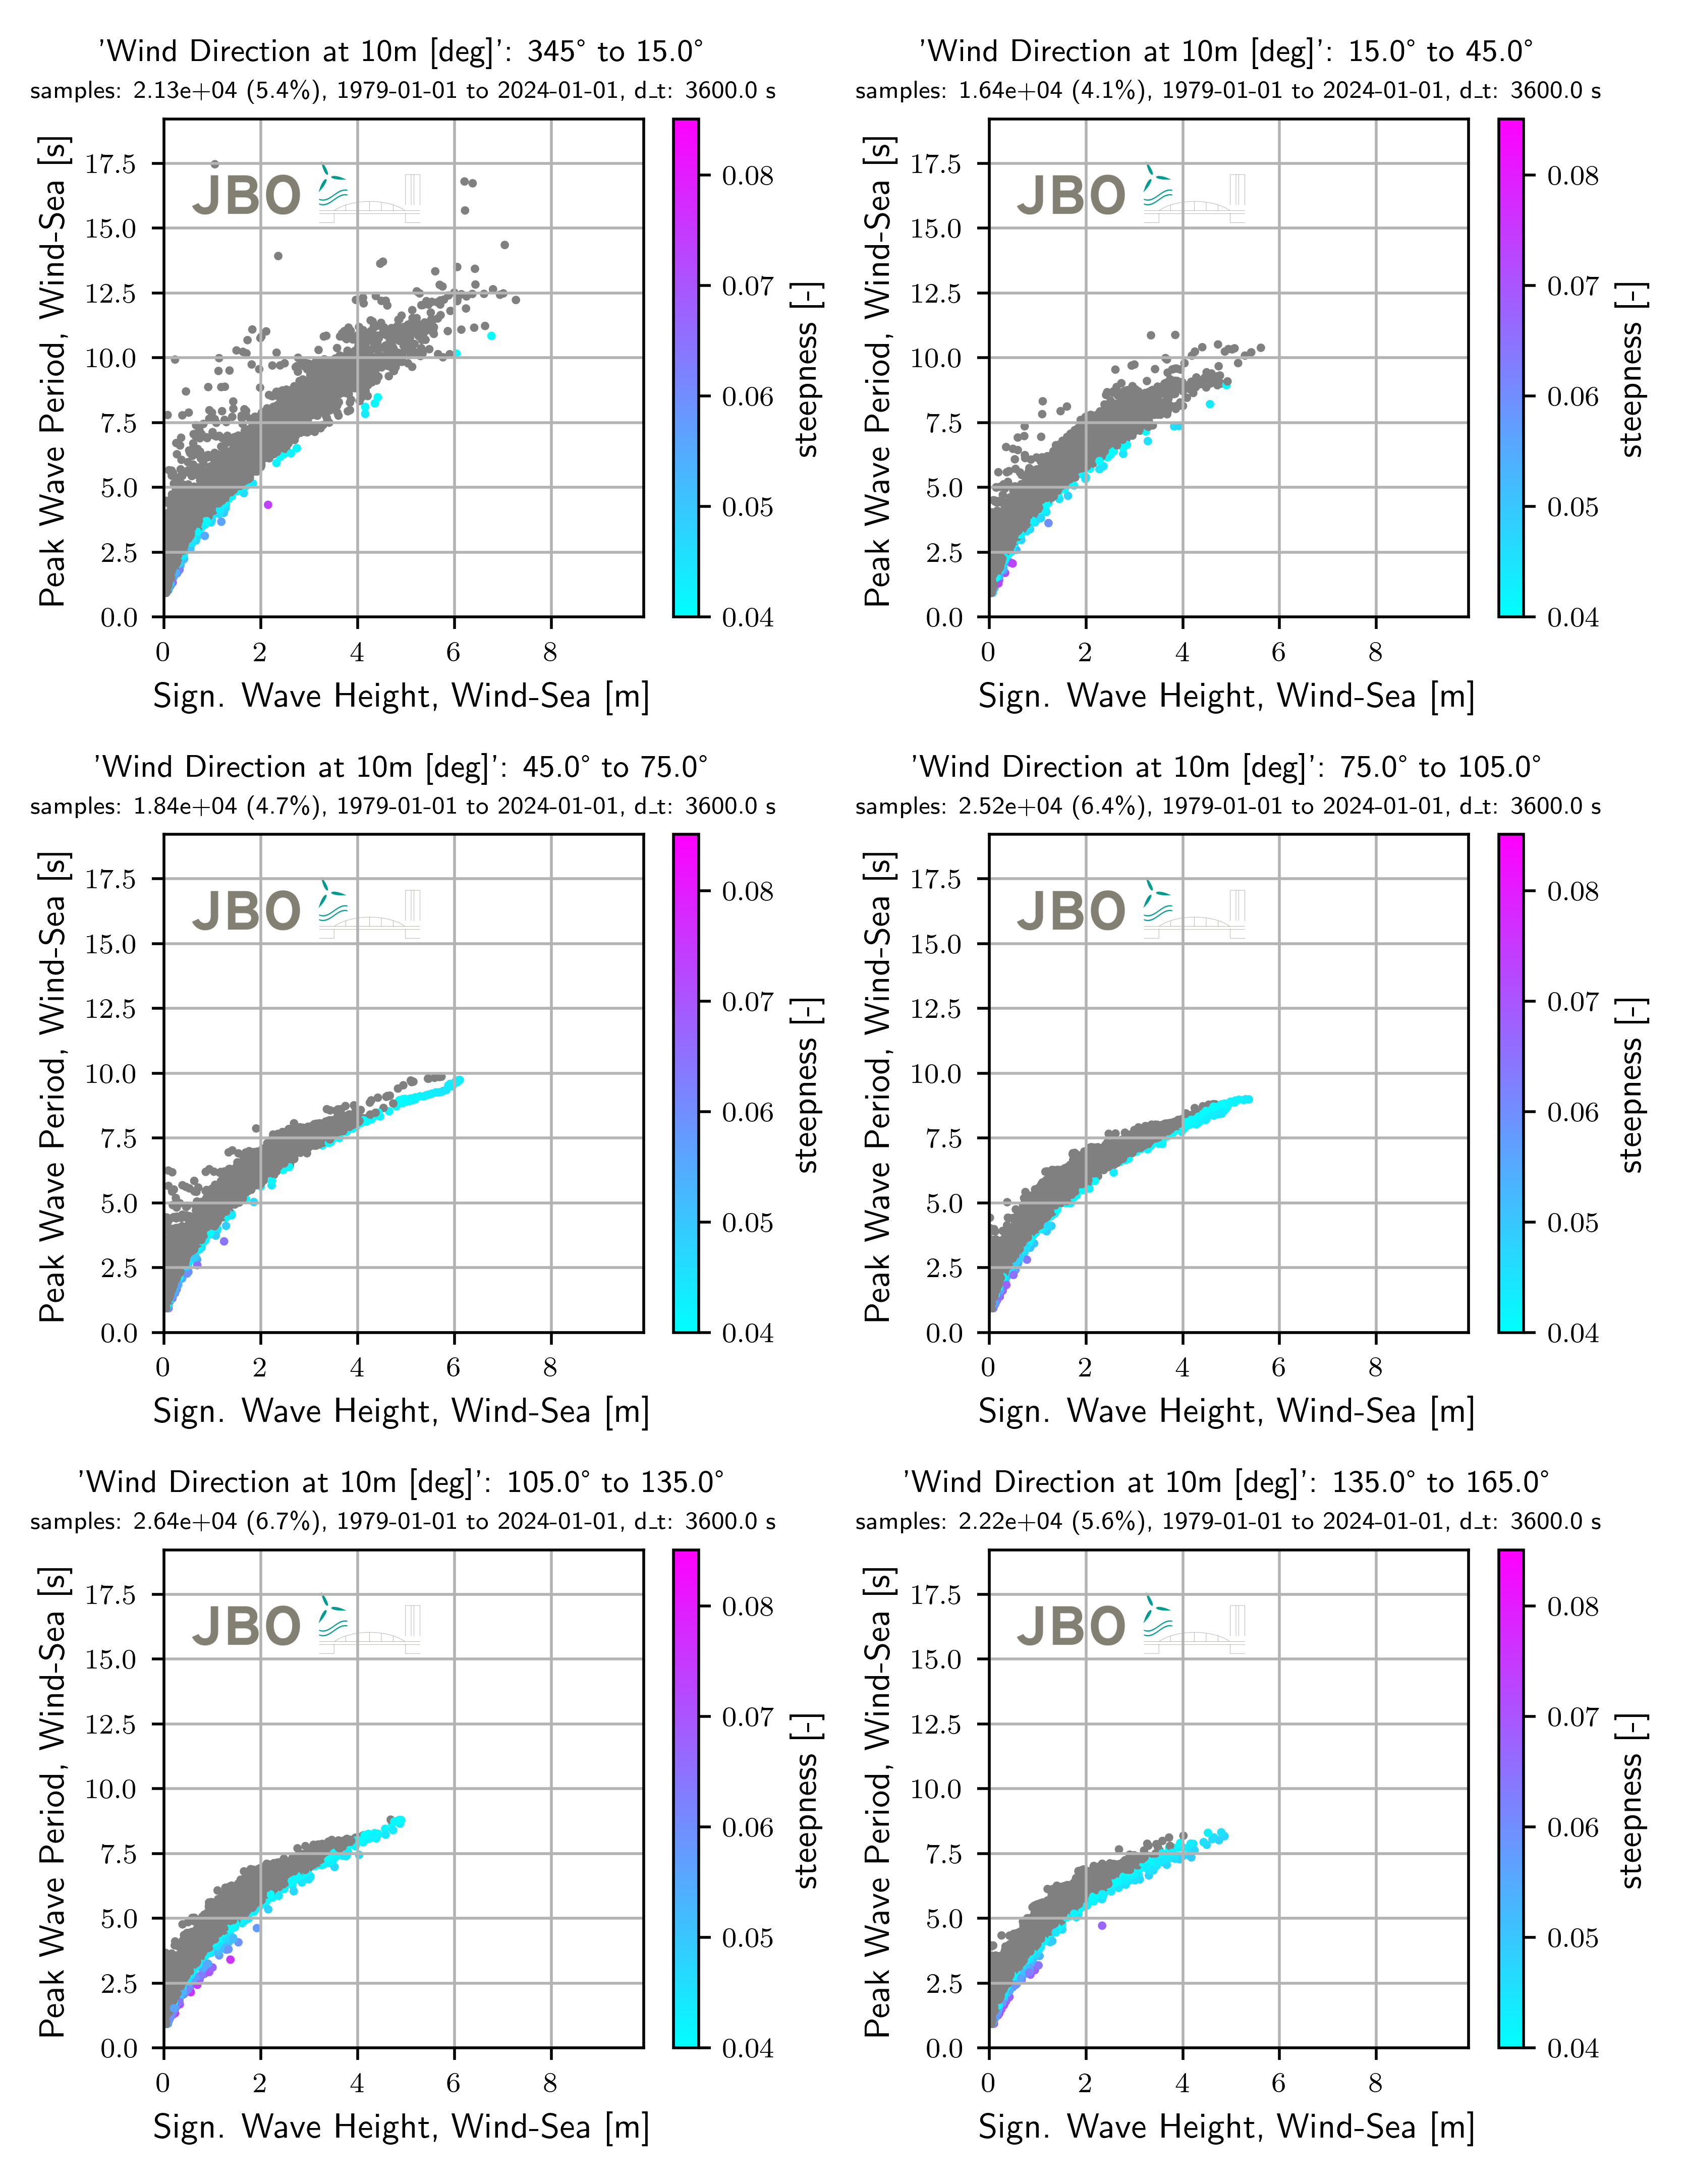
\includegraphics[width=1.0\textwidth]{C:/Users/aaron.lange/Desktop/Projekte/Hindcast_Tool/HindTool/example_output/WaveBreak_wind_page_1.png} 
 \caption{ WaveBreak-wind-page-1 } 
 \label{fig: WaveBreak_wind_page_1 } 
\end{figure}
\begin{figure}[H] 
 \centering 
 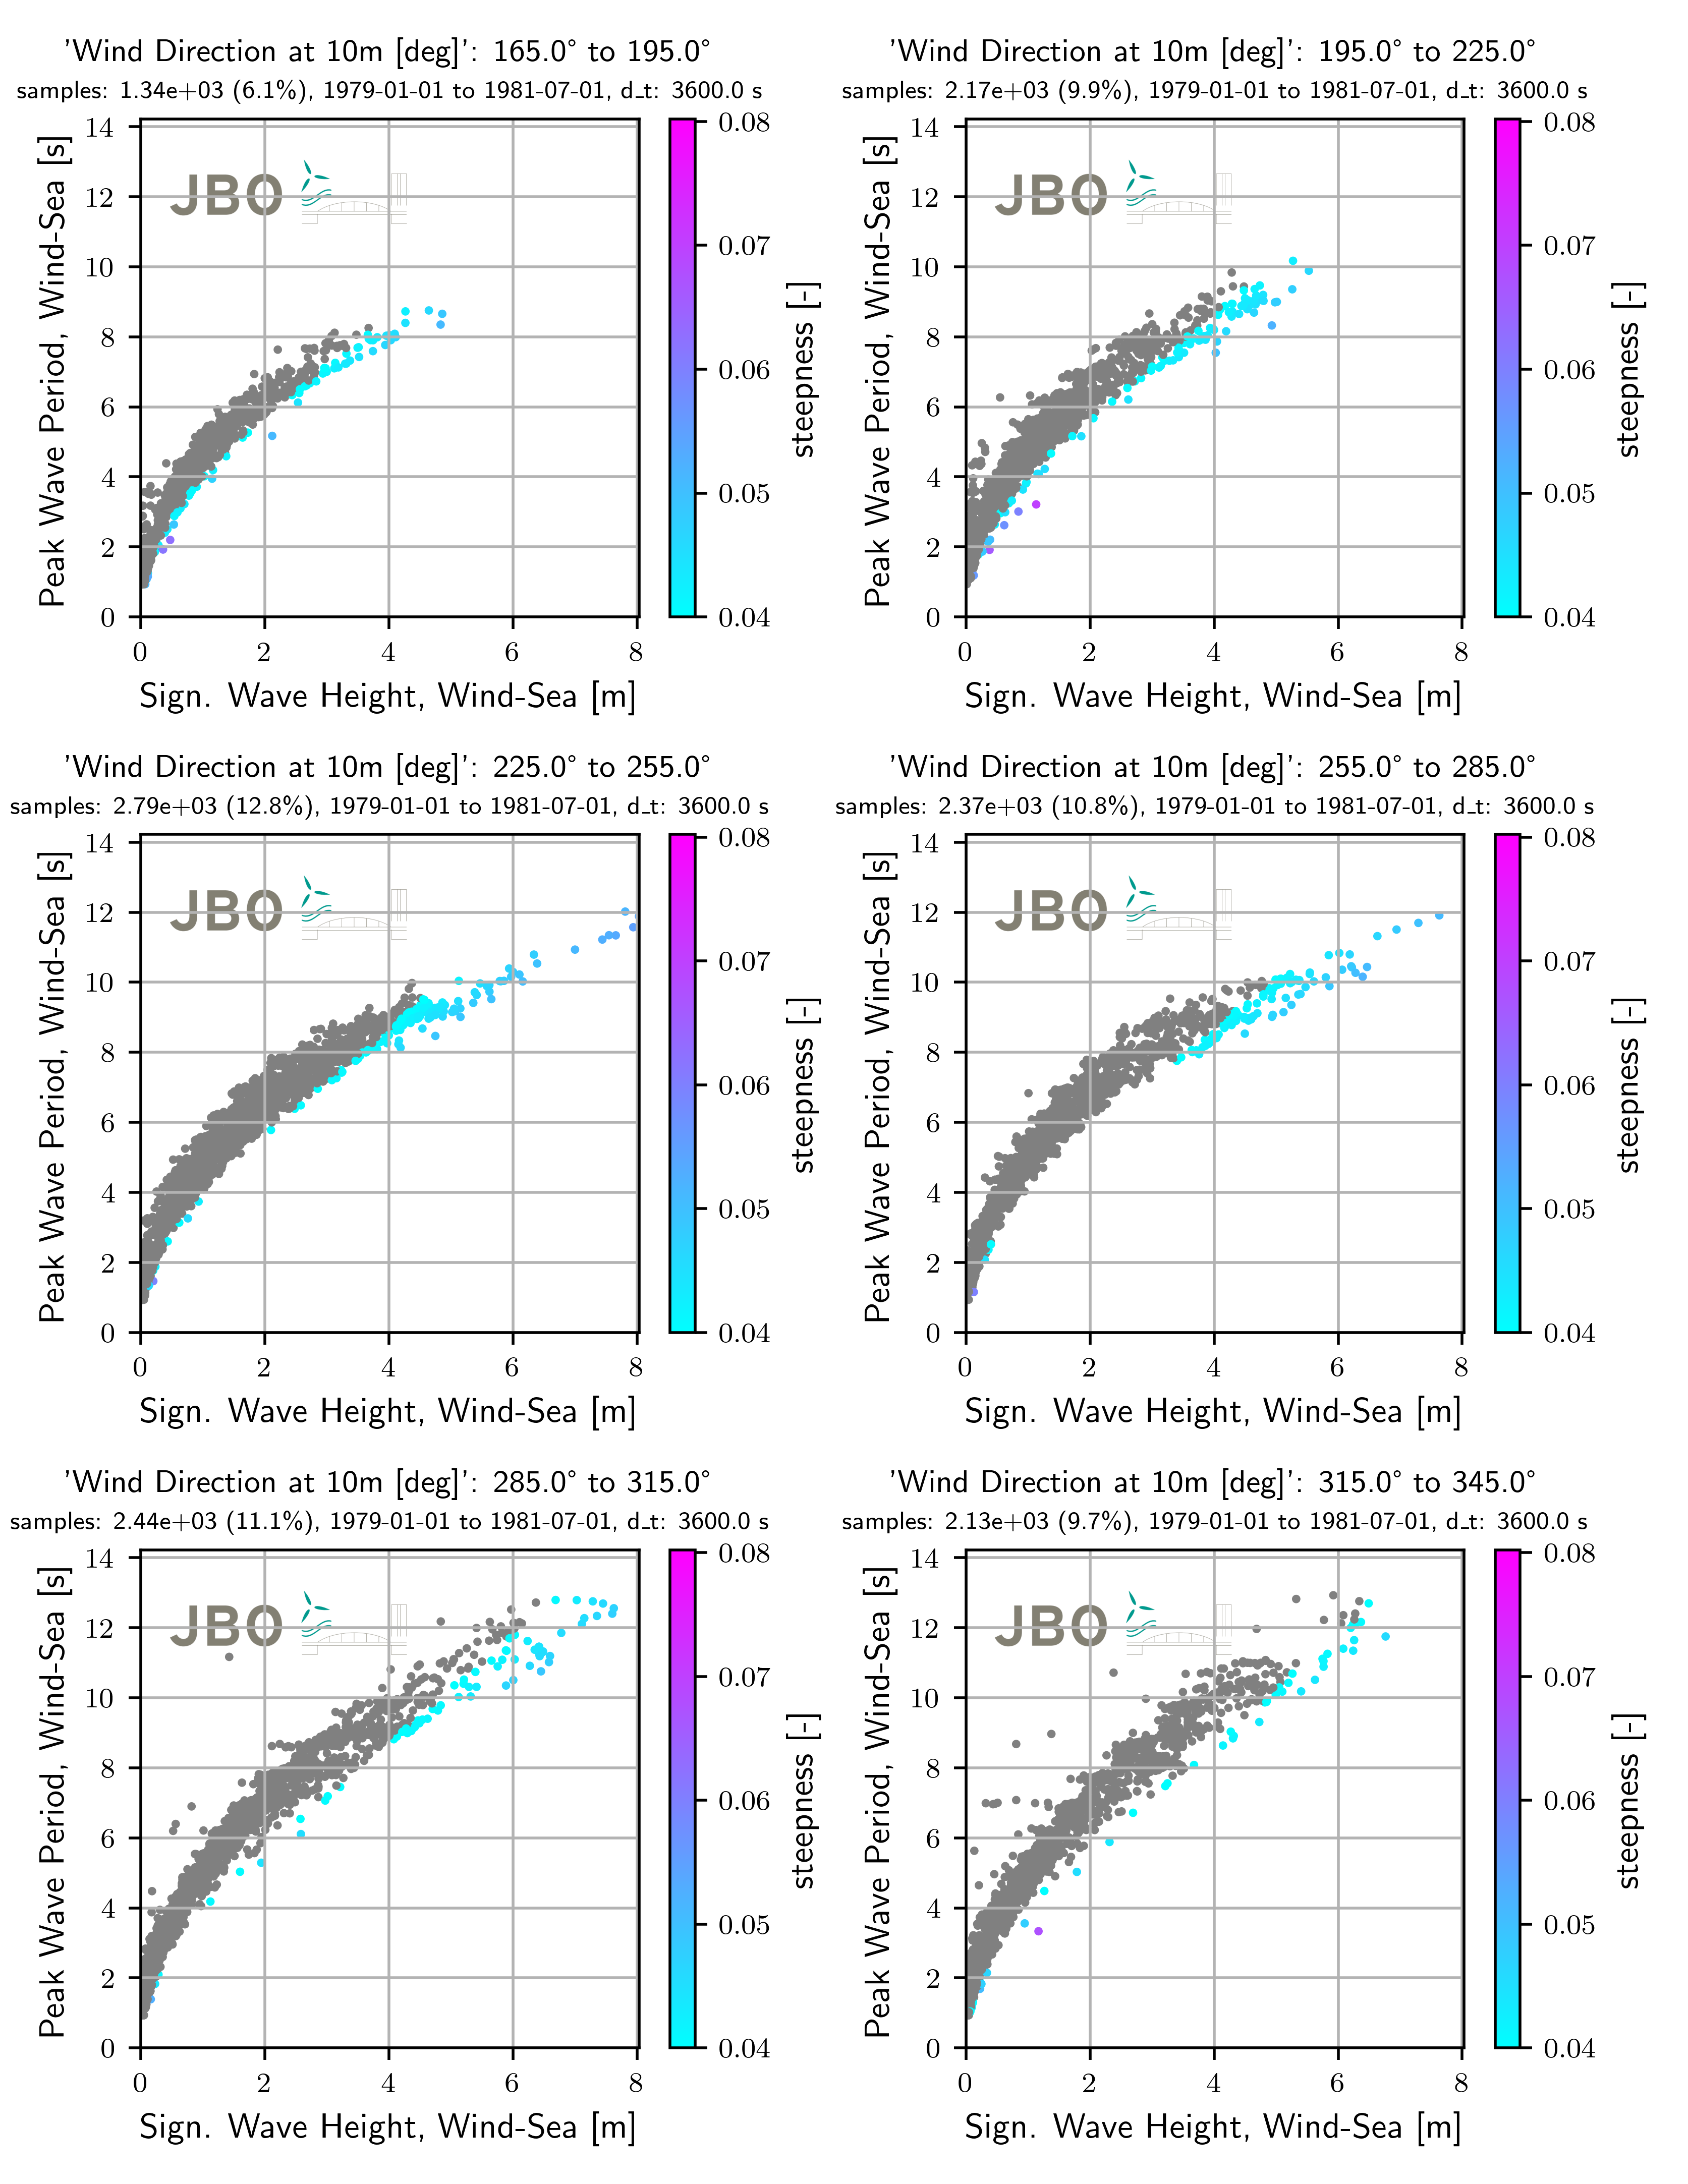
\includegraphics[width=1.0\textwidth]{C:/Users/aaron.lange/Desktop/Projekte/Hindcast_Tool/HindTool/example_output/WaveBreak_wind_page_2.png} 
 \caption{ WaveBreak-wind-page-2 } 
 \label{fig: WaveBreak_wind_page_2 } 
\end{figure}


\end{document}